\documentclass{article}
\usepackage[margin=1in]{geometry}
\usepackage{amsmath}
\usepackage{amssymb}
\usepackage{hyperref}
\usepackage{tikz}
\usepackage{graphicx}
\usepackage{placeins}
\usetikzlibrary{positioning, arrows.meta}

\title{Disentangling Shot Quality and Player Ability in Expected Goals Models (COMP 4600 Assignment 2.2 - Deliverable 1)}
\author{Daniel Elias}
\date{May 2026}

\begin{document}
\maketitle

\section{Abstract}
Expected goals (xG) has become a central statistic in modern association football (soccer) analytics, providing a probabilistic estimate of scoring a goal based on shot characteristics. Originally coming from early statistical models of shot success, it has developed into a sophisticated machine learning problem incorporating spatial and contextual features. However, there is a fundamental limitation: most xG models assume player ability is homogeneous, neglecting heterogeneity in finishing skill. This can introduce bias and limits interpretability when evaluating an individual player. However, incorporating player-specific finishing ability into xG models represents a significant algorithmic challenge due to sparse observational data, confounding between shot selection and player quality, and identifiability issues between shot quality and latent player skill.

This paper investigates whether xG models can be extended to jointly estimate shot quality and player-specific finishing ability using a hierarchical Bayesian framework. Building on foundational work in this field, including logistic regression-based models and mixed-effects models of players' scoring ability, this report formulates xG estimation as Bernoulli trials conditioned on shot characteristics and player-specific latent effects. The framework uses partial pooling in an attempt to mitigate overfitting and stabilise player estimates given the sparsity of data.

Using StatsBomb open event data from LaLiga (Spanish Tier 1), a baseline logistic regression model is implemented solely using shot distance (from the goal) and angle (to the goal) as predictors. Preliminary evaluation shows a reasonable aggregate calibration between expected goals and actual goals, but weak discriminatory performance, creating a need for richer contextual and player-specific modeling. The proposed model offers a principled method for disentangling shot quality from player-specific finishing ability while quantifying uncertainty. The paper concludes by discussing limitations of observational footballing data and future directions involving tracking data, sequential event modeling and neural embedding approaches.

\section{Motivation}
Due to the low-scoring and stochastic nature of football, quantifying a player's performance is inherently challenging, using only traditional metrics such as goals and assists. Goals are relatively rare events and strongly influenced by randomness, teammate quality, opposition strength and tactical systems. As a result of these factors, goal totals tend to fail to capture the underlying quality of a player's decision making or shot-taking ability. This caused the emergence of analytics in football and probabilistic performance metrics designed to measure the quality of scoring opportunities rather than just outcomes.

Expected Goals (xG) has become one of the most influential statistics in modern football analysis. xG models estimate the probability of a shot resulting in a goal using contextual information, such as shot distance, shot angle, body part used, defensive pressure, other players near the player, and preceding actions. Instead of analysing a player solely using goals scored, xG attempts to measure the quality of chances taken. This allows analysts to distinguish consistent performances from randomness.

The conceptual foundation of xG originates from Barnett and Hilditch\cite{barnett1993}, who proposed the concept of probabilistic possession evaluation, through the metric "Yield":
\begin{equation}
    \text{Yield} = P (\text{goal scored}) - P(\text{goal conceded})
\end{equation}
This is one of the earliest attempts to represent football as a stochastic process in which actions have expected outcomes, rather than only realised outcomes. Their work showed that approximately 10\% of shots resulted in goals, motivating the need for probabilistic models capable of estimating shot success.

Subsequent work by Ensum, Pollard and Taylor\cite{ensum2004} formalised this idea through logistic regression models of shot conversion, where each shot was treated as a Bernoulli trial, and estimated the probability of scoring based on contextual shot features, such as distance to goal, angle to goal, and defensive pressure. This established the foundation for modern xG modelling.

Modern xG models have expanded through using machine learning models and richer event datasets\cite{mead2023}. Contemporary models incorporate even more contextual features, such as whether the shot was taken with a foot, or if it was a header, as well as the current pattern of play, i.e. if it was from a counter-attack, a set-piece, or open play. Despite all these advances, most publicly available xG models still remain player-agnostic.

This assumption is problematic in practice, as elite players such as Erling Haaland or Harry Kane consistently outperform xG models based on league-average conversion rates, while worse finishers would consistently underperform expected values. As a result, traditional xG models may conflate shot quality with player finishing ability. A model which predicts an identical probability for two completely different players taking the same shot implicitly assumes that finishing ability is not a differentiating factor.

Extending xG models to account for player-specific finishing ability brings with it several computational and statistical challenges. Firstly, observational data in football is sparse: most players accumulate relatively few shots making direct estimation unstable. Secondly, player ability is confounded with shot selection, where a more skilled player may attempt more difficult shots due to their superior skill. Finally, there is an identifiability problem where shot quality and player ability may explain the same observed outcomes, as a result, separating latent finishing ability from shot quality becomes a difficult inference problem using noisy observational data.

\section{Formulation}
Consider a dataset containing individual football shots indexed by $i$. Each shot is associated with:
\begin{itemize}
    \item Player Identity $p(i)$
    \item A feature vector $\mathbf{x}_i \in \mathbb{R}^d$ (distance from goal, angle to goal, context of the shot)
    \item Binary outcome $y_i \in \{0,1\}$ (goal or miss)
\end{itemize}
Traditional xG models estimate the probability of scoring as:
\begin{equation}
    P(y_i = 1 \mid \mathbf{x}_i = \sigma(f({x}_i)))
\end{equation}
Where:
\begin{itemize}
    \item $f({x}_i)$ is a learned function representing shot quality
    \item $\sigma(\cdot)$ is the logistic function
\end{itemize}
In logistic regression models this becomes:
\begin{equation}
    p_i = P(y_i = 1 \mid {x}_i) = \frac{1}{1 + e^{-(\beta_0 + \beta^\top {x}_i)}}
\end{equation}
These models assume that player ability is homogeneous. To incorporate heterogeneity into a model, this paper expands the formulation using a latent player-specific parameter:
\begin{equation}\label{eq4}
    P(y_i = 1 \mid {x}_i, \theta_{p(i)}) = \sigma (f({x}_i) + \theta_{p(i)})
\end{equation}
Where:
\begin{itemize}
    \item $f({x}_i)$ models shot quality
    \item $\theta_{p(i)}$ models a specific player's finishing ability for a player $p(i)$
\end{itemize}
A positive $p(i)$ value indicates the specific player converts chances at a rate above the league-average, while a negative value implies a below-average rate of converting chances.

The main challenge is in identifying $\theta_{p}$ solely from observational data, specifically an identifiability problem:
\begin{equation} \label{xgpi}
f(\mathbf{x}_i) + \theta_{p(i)} \approx f'(\mathbf{x}_i),
\end{equation}\label{eq5}
Where multiple paramterisations may lead to the same proabilistic likelihood. That is, given that the probability of a goal is $\theta(2.0)$, that could be obtained from:
\begin{itemize}
    \item $f = 2.0,$ $\theta = 0.0$
    \item $f = 0.5,$ $\theta = 1.5$
\end{itemize}
For example, a high probability to score may arise from:
\begin{itemize}
    \item an independently high-quality shot, such as a ``tap in"
    \item an elite finisher being able to convert difficult shots
    \item a combination of the previous two things
\end{itemize}
This ambiguity makes it difficult to distinguish player ability from shot quality. 

This issue is further exacerbated by:
\begin{itemize}
    \item \textbf{Data Sparsity}: the majority of players have limited shot samples, particularly defenders and substitutes. Estimating player ability from limited samples can lead to highly variable estimates.
    \item \textbf{Confounding}: A player's ability and confidence in shooting affects which shots they take. Elite finishers may intentionally attempt more difficult shots due to their superior ability, leading to observed shot distributions not being independent of player ability.
    \item \textbf{Selection bias}: Only shots within a dataset are modeled. A tactical system may affect which shots are taken, as xG models only estimate the probability of realised shots, not all positions from where a player could take a shot.
\end{itemize}

\section{Methodology}
\subsection{Baseline Model}
As a benchmark for comparison, we first define a standard player-agnostic baseline using logistic regression. Each shot is modeled as an independent Bernoulli trial dependent on spatial features:
\begin{equation}
    y_i \sim \text{Bernoulli}(p_i)
\end{equation}
The baseline model defines the probability of a successful shot, $p_i$, through the standard logistic link function:
\begin{equation}
    p_i = \sigma(\beta_0 + \beta^\top \mathbf{x}_i) = \frac{1}{1 + e^{-(\beta_0 + \beta^\top \mathbf{x}_i)}}
\end{equation}
where $\beta_0 \in \mathbb{R}$ represents the global intercept and $\beta \in \mathbb{R}^d$ represents the vector of structural coefficients. Following from the foundational geometric principles of football analytics established by Ensum, Pollard and Taylor \cite{ensum2004}, the feature vector $x_i$ is constructed using core spatial attributes derived from raw $(x, y)$ coordinates:
\begin{itemize}
    \item Distance to goal, $(d_i)$: the Euclidean distance from the shot origin to the centre of the goal, which is located at $(120,40)$, and formulated as:
    \begin{equation}
        d_i = \sqrt{(120 - x_i)^2 + (40-y_i)^2}
    \end{equation}
    \item Shot angle, $\alpha_i$ formulated as:
    \begin{equation}
        \text{Shot location: } S_i = (x_i, y_i)
    \end{equation}
    \begin{equation}
        \text{Location of the two goalposts: } L = (120, 40 - \frac{w}{2})\text{, }R = (120, 40 + \frac{w}{2})
    \end{equation}
    Where $w$ is the width of the goal, 7.32.
    \begin{equation}
        a_i = || S_i - L|| \text{, } b_i = ||S_i - R||
    \end{equation}
    Which gives the angle to the goal formula:
    \begin{equation}
        \alpha_i = cos^{-1}(\frac{a_i^2 + b_i^2 - w^2}{2a_ib_i})
    \end{equation}
\end{itemize}

\subsection{Hierarchical Bayesian Extension}
In an attempt to decouple individual skill from a lucky opportunity, we expand the model by embedding a latent, unobserved random effect $\theta_{p(i)}$ specific to each player:
\begin{equation}
    logit(p_i) = log(\frac{p_i}{1 - p_i}) = \beta_0 + \beta^\top x_i + \theta_p(i)
\end{equation}
Where:
\begin{itemize}
    \item $\beta_0$ is the baseline probability, if all features were weighted to 0
    \item $\beta^\top x_i$ is the transpose of the weight vector
    \item $\theta_{p(i)}$ is the player's individual finishing deviation
\end{itemize}
This follows on from equation \ref{eq4}, where $f(x_i)$ is modeled by the baseline probability and the transpose of the weight vector.

Estimating independent parameters for every single player via fixed-effects introduces severe overfitting and high variance due to data sparsity, as few players take the majority of shots. This is resolved by using partial pooling within a hierarchical structure:
\begin{equation}
    \theta_p \sim \mathcal{N}(0, \sigma_\text{player}^2), \forall p \in \{1, ..., P\}
\end{equation}
\begin{equation}
    \sigma_\text{player} \sim \text{Exponential}(\lambda)
\end{equation}
This hierarchical structure shares statistical strength across the entire population of players who have taken a shot. It regularises individual estimates based on sample size where players who take a large amount of shots deviate from the league average if the data supports it, but low-volume shooters tend towards the average $(\theta \to 0)$.

\subsubsection{Identifiability}
A core challenge within this model is identifiability, as shown previously in equation \ref{eq5}. In this model, by penalising extreme and implausible player deviations, the model prevents $\theta_{p(i)}$ from being effected by high variance, thereby stabilising the model and ensuring the parameters remain interpretable.

\subsection{Data Collection and Inference}
The model was implemented using publicly available StatsBomb open event data, specifically from LaLiga (Spanish First Division) from the 2004/05 season to the 2020/21 season. StatsBomb was chosen due to its high shot samples from multiple consecutive seasons, as well as its highly-specific annotations. The data pipeline filters out all non-shot actions, normalises spatial coordinates and calculates the distance to goal and shot angle, as well as creating binary goal indicators $y_i \in \{0, 1\}$.

Posterior inference was executed in PyMC using the No-U-Turn Sampler (NUTS), which is a more advanced variant of the Hamiltonian Monte Carlo (HMC). Rather than calculating unstable point values, NUTS samples from the full joint posteriror of the paramters:
\begin{equation}
    P(\beta, \theta, \sigma_{\text{player}} \mid \mathcal{D}) \propto P(\mathcal{D} \mid \beta, \theta, \sigma_{\text{player}}) \, P(\beta) \, P(\mathbf{\theta} \mid \sigma_{\text{player}}) \, P(\sigma_{\text{player}})
\end{equation}
Posterior means are then used as localised parameter estimates, while credible intervals provide a direct measure of statistical uncertainty. This framework offers a key advantage over deterministic machine learning approaches by explicitly capturing uncertainty in estimates.

\section{Results}
\subsection{Experiment Design}
The experiment was designed as a comparative study between two different probabilistic models. A baseline model, which is a logistic regression based on shot angle and shot distance, and a player-specific model, which incorporates the parameters of the first along with individual player finishing ability. This structure essentially acts as an A/B test, as the only difference between the two is the player ability, that is, there is no further context included in the player-specific model.
\subsubsection{Baseline Model}
First, we must establish that the baseline model accurately captures the difficulty of a shot. Using these two figures:

\begin{figure}[htbp]
    \centering
    \begin{minipage}{0.48\linewidth}
        \centering
        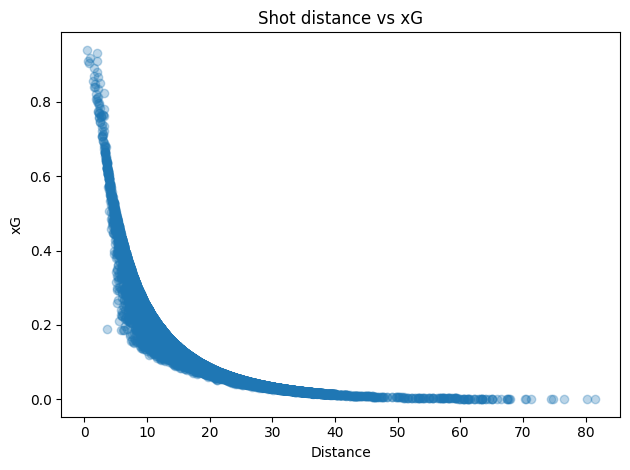
\includegraphics[width=\linewidth]{distance_xg.png}
        \caption{Shot distance compared to xG}
        \label{fig:distance_xg}
    \end{minipage}
    \hfill
    \begin{minipage}{0.48\linewidth}
        \centering
        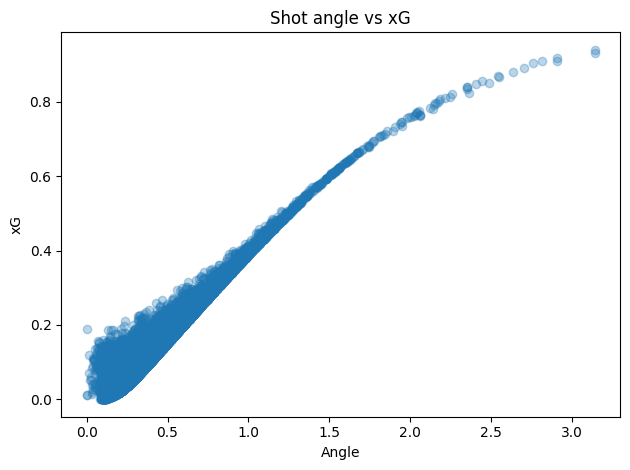
\includegraphics[width=\linewidth]{angle_xg.png}
        \caption{Shot angle compared to xG}
        \label{fig:angle_xg}
    \end{minipage}
\end{figure}
\FloatBarrier
We can see that there are clear relationships between shot distance and xG, and shot angle and xG. For shot distance, you can see that xG exponentially decays as distance increases, implying that shots from further out are more difficult. For shot angle, you can see as the angle gets 'better', xG scales logically. We can further reinforce these baseline findings using a heatmap:

\begin{figure}[htbp]
    \centering
    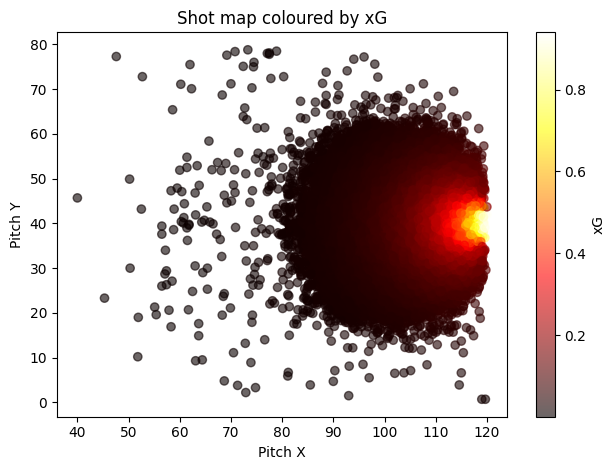
\includegraphics[width=0.5\linewidth]{xg_heatmap.png}
    \caption{Heatmap showing xG of a shot compared to location on a pitch}
    \label{fig:xg_heatmap}
\end{figure}
\FloatBarrier

From this we can see that the closer a shot is to goal, and the more direct the angle, the higher likelihood it is that it will result in a goal.
This closely aligns with real-world football intuition, as well as typical scoring patterns. Dangerous chances generally come from close-range central positions where goalkeepers will have less reaction time, and attackers will have wider goal visibility. The baseline model shows a strong foundational estimate of shot quality from just these two parameters.

\begin{figure}[htbp]
    \centering
    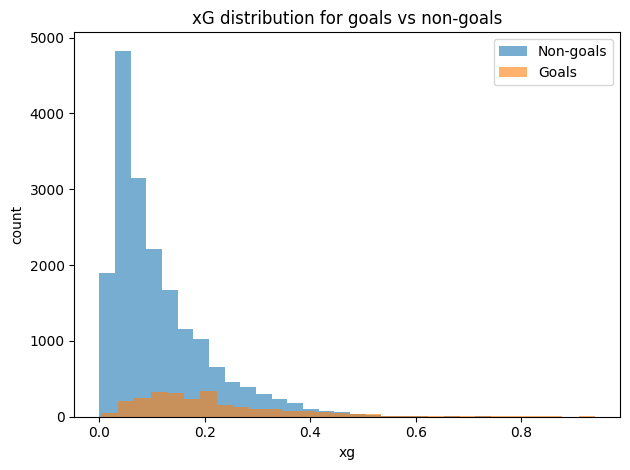
\includegraphics[width=0.5\linewidth]{calaibration.png}
    \caption{Non-goal shots xG vs goal shots xG}
    \label{fig:calibration_base}
\end{figure}
\FloatBarrier

This figure provides additional confirmation of the validity of the baseline model by comparing the distribution of xG values for non-goal shots versus goal shots. It shows that goals are disproportionately associated with higher xG probabilities, while shots that did not result in goals cluster more tightly around the lower xG range. This indicates simply using distance and angle can separate dangerous and non-dangerous chances decently well. However, there is still overlap between the two distributions, which implies that there are further factors that affect the success of a shot, not just distance and angle, which is where player-specific xG comes in.

\subsubsection{Player-Specific Model}
After verifying the validity of the baseline model, the experiment introduces player-specific finishing parameters to test whether individual skill can meaningfully affect predictive performance. The hypothesis is that elite players consistently outperform average shot conversion rates implied by shot geometry alone. I also removed the players whose sample size was so low there was a great amount of uncertainty, so as to not skew the results. 

\begin{figure}[htbp]
    \centering
    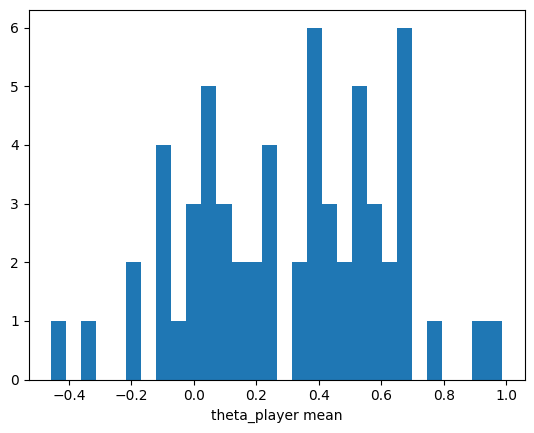
\includegraphics[width=0.5\linewidth]{theta_player.png}
    \caption{Estimated player finishing coefficients}
    \label{fig:theta_player}
\end{figure}
\FloatBarrier
The figure above shows coefficients learned by the model. They are centred near-zero, representing average finishing ability across the population, however, it shows substantial positive and negative deviations, indicating a large variation in player ability in finishing. Positive coefficients correspond to players who convert chances at above league-average rates, while negative coefficients represent below-average finishers.

The distribution is also continuous, which implies that finishing skill is a spectrum, and not a binary value of elite/non-elite.

A key strength of the experiment design is it also evaluates the uncertainty around the finishing ability estimates as shown:
\begin{figure}[htbp]
    \centering
    \begin{minipage}{0.48\linewidth}
        \centering
        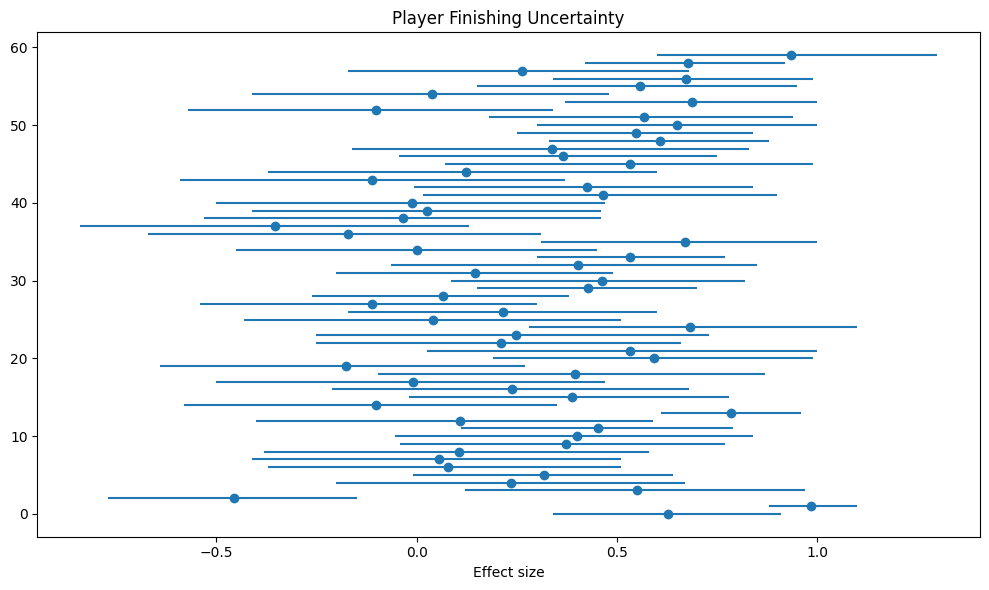
\includegraphics[width=\linewidth]{finishing_uncertainty.png}
        \caption{Player finishing uncertainty}
        \label{fig:finishing_uncertainty}
    \end{minipage}
    \hfill
    \begin{minipage}{0.48\linewidth}
        \centering
        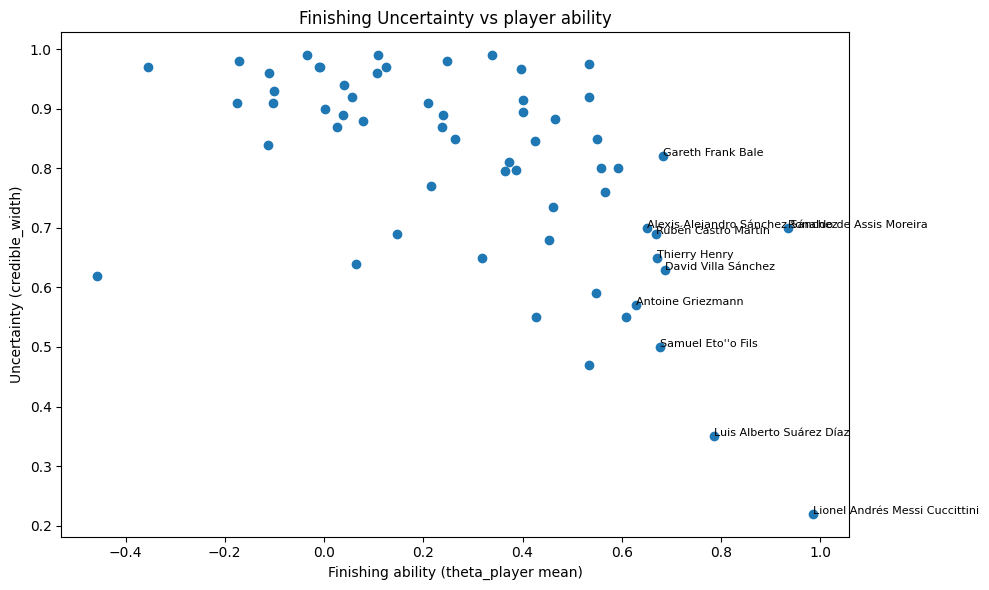
\includegraphics[width=\linewidth]{player_scatter.png}
        \caption{Player-specific ability compared to uncertainty}
        \label{fig:player_scatter}
    \end{minipage}
\end{figure}
\FloatBarrier
Players with a large sample size of shots tend to have lower uncertainty as the model has more evidence to support their coefficient. Elite players, such as Lionel Messi, show both high finishing coefficients and low uncertainty, indicating that his overperformance of base xG is due to consistent, superior finishing ability instead of a lucky shot. Without uncertainty analysis, isolated purple patches or small anomalies could be incorrectly classified as genuinely elite finishing ability. By incorporating this, it strengthens the validity of this experiment.

\subsection{Results and Observations}
The comparison between the baseline and player-specific models reveals several findings on finishing skill and probability estimation.

One of the clearest observations emerges from these two figures:
\begin{figure}[htbp]
    \centering
    \begin{minipage}{0.48\linewidth}
        \centering
        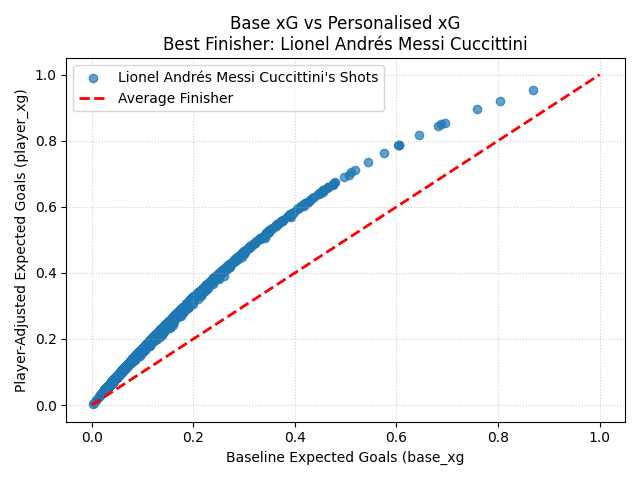
\includegraphics[width=\linewidth]{best_finisher_xg.png}
        \caption{Personalised xG vs Base xG for Lionel Messi}
        \label{fig:best_finisher_xg}
    \end{minipage}
    \hfill
    \begin{minipage}{0.48\linewidth}
        \centering
        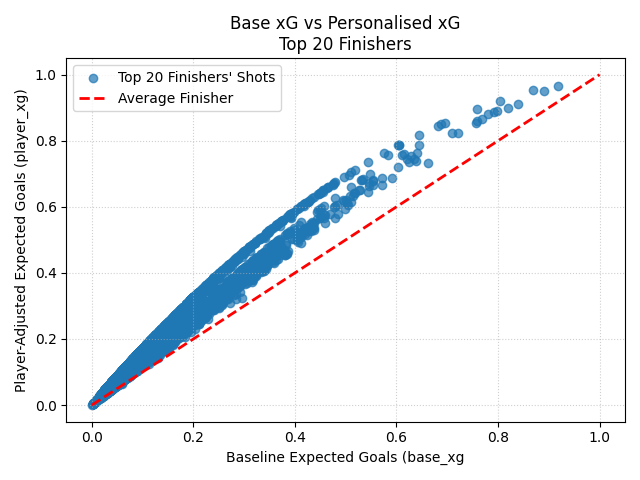
\includegraphics[width=\linewidth]{top_20_xg.png}
        \caption{Personalised xG vs Base xG for top 20 finishers}
        \label{fig:top_20_xg}
    \end{minipage}
\end{figure}
\FloatBarrier
These figures show the baseline xG compared to the player-adjusted xG for the most elite finishers. The dashed red line represents the expectation of the ``average" player, where deviations above the line indicate greater-than-average skill. For the best players, their reference points are consistently above the ``average'' player's line, which shows the model systematically increases the probability of shots taken being scored by the elite finishers. For example, Messi taking a shot that is usually worth 0.2xG, might be adjusted to be worth 0.3xG when he takes it, which is a significant difference in the likelihood of that shot going in, which implies that the same chance can have different scoring probabilities based on who is taking the shot. Interestingly, the lines start to converge as the baseline xG increases, which suggests that they are unlikely to reach a probability of 1 when the baseline probability is less than 1.

This directly challenges the assumption that xG models should be entirely context-independent, and supports the idea that finishing ability is measurable and predictive.

The next figure ranks players according to their finishing coefficients on a log-odds scale:
\begin{figure}[htbp]
    \centering
    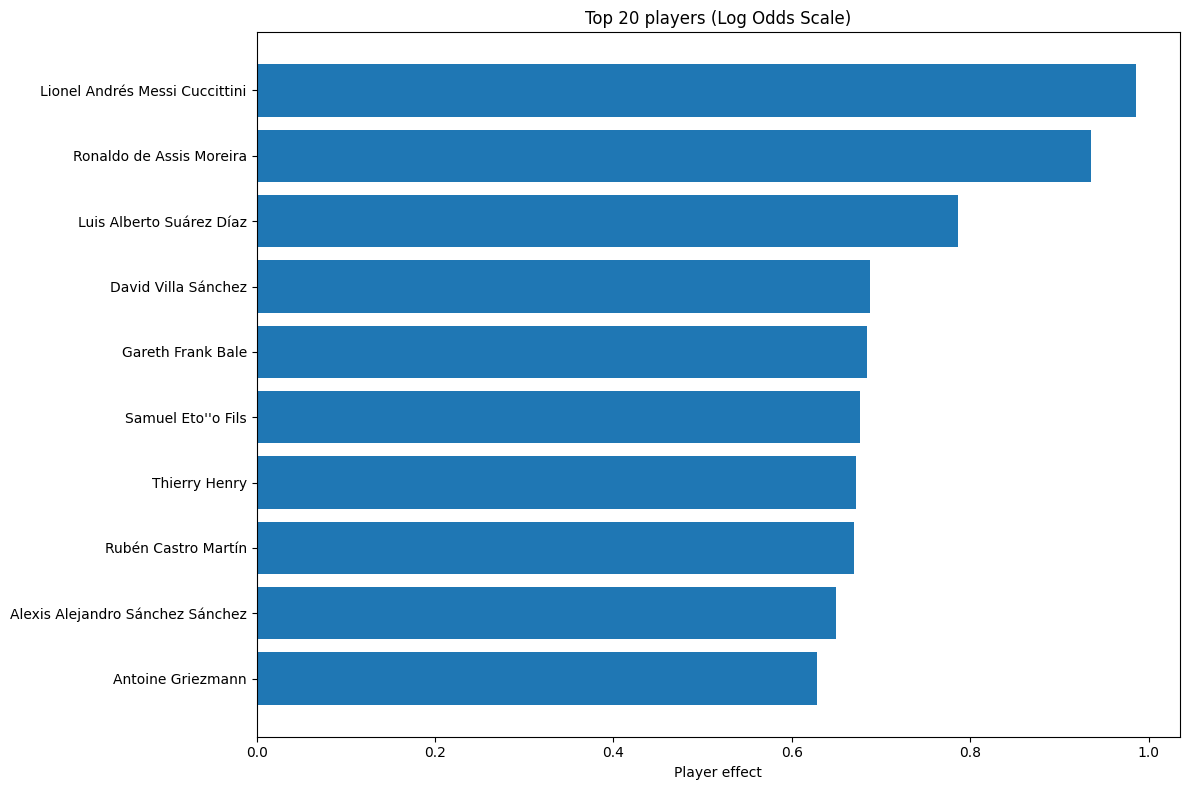
\includegraphics[width=0.5\linewidth]{top_10_players.png}
    \caption{Log-Odds Scale of top 10 finishers}
    \label{fig:top_10_xg}
\end{figure}
\FloatBarrier
Notably, the model identifies historically recognised elite finishers such as Lionel Messi, Ronaldinho and Luis Suarez. This helps reinforce the fact the model works as it was not trained to recognise the names of famous players. This provides strong validity for the model and suggests the learned parameters correspond to genuine football ability.

\subsection{Model Comparison}
To determine whether the player-specific model is superior than the baseline model for modeling xG it is necessary to evaluate the models using metrics designed for probabilistic prediction tasks.

Log loss was used as the primary metric as shot outcomes are binary, but the model outputs probabilities between 0 and 1. Log loss rewards accurate estimates, but heavily penalises predictions that are confidently incorrect. This is important as xG is used to model the likelihood of a shot resulting in a goal. The baseline model achieved a Log Loss of 0.3193, while the player-specific model had a log loss of 0.3057. Even though the absolute difference is relatively minor, even small reductions of Log Loss can be significant because they reflect consistent improvement across thousands of observations, which indicates the player-specific model produces more realistic probability estimates.

ROC-AUC was used to measure each model's ability to distinguish goals from non-goals. AUC measures how often the model assigns a higher xG value to a goal than to a missed shot. The baseline model achieved an AUC of 0.7475, which improved to 0.7802 after accounting for player-specific ability. This suggest the player-specific model is better at identifying genuinely dangerous chances and supports the hypothesis that finishing ability provides better predictive information beyond shot location alone.

The Brier Score evaluated calibration through measuring the mean-squared difference between predicted probabilities and actual outcomes. Although the score lowered between the models, from 0.0985 to 0.0942, both models have highly accurate prediction.

Finally, I decided to check the totals of the xG calculated, compared to the actual number of goals scored, which resulted in the baseline model predicting 2685 goals  scored, and the player specific model predicting 2653.7 goals scored. The actual number of goals scored was 2653, showing the player-specific model was highly accurate, although both models have strong overall calibration.

\subsection{Project Artifact Link}
\url{https://gitlab.comp.anu.edu.au/u8303341/comp4600-assignment2.2}

\section{Conclusion and Discussion}
The results show that incorporating player-specific finishing effects improves expected goals modeling in a statistically meaningful way. The baseline model effectively captures the physical difficulty of shots through distance and angle; however, the player-specific model builds upon this foundation by isolating and quantifying individual finishing skill.

Across every single major metric the player-specific model outperformed the baseline:
\begin{itemize}
    \item Lower Log Loss indicates more accurate probability assignments
    \item Higher ROC-AUC shows superior discrimination between goals and non-goals
    \item Lower Brier Score confirms improved calibration
    \item Near-perfect totals shows remarkable accuracy on a macro-level
\end{itemize}
Additionally, the visualisations reveal that elite players consistently outperform baseline expectations in repeatable and statistically reliable ways.

Combining these findings support the conclusion that finishing ability is not purely random in an xG model, but a measurable and predictive component. The player-specific xG model thus provides a more realistic and powerful framework for evaluating shot quality and finishing ability.

\subsection{Limitations}
The main limitation was the availability of event data in football matches. Although the StatsBomb dataset used covered 17 seasons of LaLiga, it only contained roughly 860 matches total. When a normal LaLiga season has 380 matches, you can see the sparsity of data. In order to alleviate this, you could pay for access to more StatsBomb data, or from another provider such as Opta. However, the cost of this can range from the tens of thousands to the millions of dollars making it infeasible for such a small study.

In addition to the limited dataset, elite players tend to take more shots than worse players, leading to much richer data being available for them and having more stable coefficients, but most players have relatively few shots. This can lead to overconfidence in rankings.

We also didn't include any extra context related to the shot, such as defensive pressure or goalkeeper positioning, which could be misattributed to player skill rather than unobserved context.

Finally, the model also assumes a player's skill is constant, and doesn't change with age, varying tactics or even injury. A single coefficient for each player may oversimplify such a dynamic attribute.

\subsection{Further Improvements}
In the future, this could be improved by providing richer contextual data for each shot, such as defensive pressure, location of players near the shot-taker, and which part of the body the shot was taken with.

Using richer and more up-to-date datasets will also improve the accuracy of the model used. Alternatively, expanding the model to different leagues such as the Premier League and Serie A could help produce more accurate coefficients.

Finally, it may be better to model more than one coefficient per player, keeping track of the manager they are playing under, tactics used, their injuries and potentially psychological effects in their personal life could lead to better, more personalised xG estimates.

\bibliographystyle{plain}
\begin{thebibliography}{9}
\bibitem{barnett1993}
V. Barnett and S. Hilditch.
\newblock The effect of an artificial pitch surface on home team performance in football.
\newblock Journal of the Royal Statistical Society: Series A, 1993.
\bibitem{ensum2004}
J. Ensum, R. Pollard, and S. Taylor.
\newblock Applications of logistic regression to shots at goal in association football.
\newblock Journal of Sports Sciences, 2004.
\bibitem{mead2023}
J. Mead, A. O’Hare, and P. McMenemy.
\newblock Expected goals in football: Improving model performance and demonstrating value.
\newblock PLOS ONE, 2023.
\end{thebibliography}

\end{document}
